\documentclass[a4paper, 11pt]{article}
\usepackage{geometry}
\usepackage{graphicx}
\usepackage{a4wide}
\usepackage{ulem}
\usepackage{amsthm}
\usepackage{amsmath}
\usepackage{amsfonts}
\usepackage{amssymb}
\usepackage[T1]{fontenc}
\usepackage{ngerman}
\usepackage{graphicx}
\usepackage{epic}
\usepackage{enumerate}
\usepackage{tabu}
\usepackage [latin1]{inputenc}
\geometry{a4paper,left=15mm,right=25mm,top=10mm,bottom=15mm}
%\renewcommand{\baselinestretch}{1.5}
\newcommand{\ol}{\overline}
\newcommand{\makeline}{\hrule\vspace{5pt}}
\newcommand{\ip}[2]{\left< #1, #2 \right>}

\title{5. �bungsblatt zu Software Qualit�t}
\author{Michel Meyer, Manuel Schwarz}

\begin{document}
  \maketitle

  \section*{Aufgabe 5.1}
  \subsection*{(a)}
  %\begin{figure}
		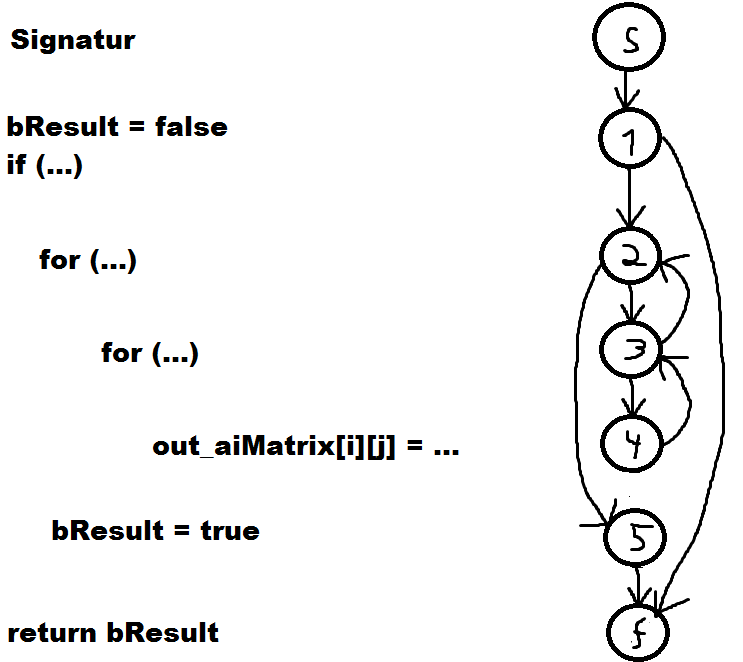
\includegraphics[width=\columnwidth]{Aufg1a.png}
	%\end{figure}
  

  \subsection*{(b)}
  \begin{tabular}[c]{|l|l|l|}\hline
  \textbf{Kategorie} & \textbf{ID} & \textbf{Pfad} \\\hline\hline
  Ohne     & A0 & $n_s, n_1, n_2, n_5, n_f$ \\\hline
  Schleife & B0 & $n_s, n_1, n_f$ \\\hline\hline
  Boundary & A1a& $n_s, n_1, n_2, n_3, n_4, n_3, n_2, n_5, n_f$ \\\hline
  Test     & A1b& $n_s, n_1, n_2, n_3, n_2, n_5, n_f$ \\\hline\hline
  Interior & A2c& $n_s, n_1, n_2, n_3, n_2, n_3, n_2, (n_3, (n_4, n_3)^k n_2)^m, n_5, n_f$ \\\hline
  Tests    & A2d& $n_s, n_1, n_2, n_3, n_2, n_3, n_4, n_3, n_2, (n_3, (n_4, n_3)^k n_2)^m, n_5, n_f$ \\\hline
           & A2e& $n_s, n_1, n_2, n_3, n_2, n_3, n_4, n_3, (n_4, n_3)^i, n_2, (n_3, (n_4, n_3)^k n_2)^m, n_5, n_f$ \\\hline
           & A3c& $n_s, n_1, n_2, n_3, n_4, n_3, n_2, n_3, n_2, (n_3, (n_4, n_3)^k n_2)^m, n_5, n_f$ \\\hline
           & A3d& $n_s, n_1, n_2, n_3, n_4, n_3, n_2, n_2, n_3, n_4, n_3, n_2, (n_3, (n_4, n_3)^k n_2)^m, n_5, n_f$ \\\hline
           & A3e& $n_s, n_1, n_2, n_3, n_4, n_3, n_2, n_3, n_4, n_3, (n_4, n_3)^i, n_2, (n_3, (n_4, n_3)^k n_2)^m, n_5, n_f$ \\\hline
           & A4c& $n_s, n_1, n_2, n_3, n_4, n_3, n_4, n_3, (n_4, n_3)^i, n_2, n_3, n_2, (n_3, (n_4, n_3)^k n_2)^m, n_5, n_f$ \\\hline
           & A4d& $n_s, n_1, n_2, n_3, n_4, n_3, n_4, n_4, (n_4, n_3)^i, n_2, n_2, n_3, n_4, n_3, n_2, (n_3, (n_4, n_3)^k n_2)^m, n_5, n_f$ \\\hline
           & A4e& $n_s, n_1, n_2, n_3, n_4, n_3, n_4, n_3, (n_4, n_3)^i, n_2, n_3, n_4, n_3, (n_4, n_3)^j, n_2, (n_3, (n_4, n_3)^k n_2)^m, n_5, n_f$ \\\hline
  \end{tabular}\\\\
  
	\noindent Erl�uterungen:\\
	\begin{tabular}[c]{|l|l|l|}\hline
	\textbf{ID} & \textbf{1. Schleifendurchlauf �u�ere Schleife} & \textbf{2. Schleifendurchlauf �u�ere Schleife} \\\hline\hline
	A2c         & 0x innere Schleife                             & 0x innere Schleife                             \\\hline
	A2d         & 0x innere Schleife                             & 1x innere Schleife                             \\\hline
	A2e         & 0x innere Schleife                             & mindestens 2x innere Schleife                  \\\hline
	A3c         & 1x innere Schleife                             & 0x innere Schleife                             \\\hline
	A3d         & 1x innere Schleife                             & 1x innere Schleife                             \\\hline
	A3e         & 1x innere Schleife                             & mindestens 2x innere Schleife                  \\\hline
	A4c         & mindestens 2x innere Schleife                  & 0x innere Schleife                             \\\hline
	A4d         & mindestens 2x innere Schleife                  & 1x innere Schleife                             \\\hline
	A4e         & mindestens 2x innere Schleife                  & mindestens 2x innere Schleife                  \\\hline
	\end{tabular}\\\\
	
	\noindent Hinter jeder Kombination steht der Term $(n_3, (n_4, n_3)^k n_2)^m$, damit nach den ersten beiden Schleifendurchl�ufen der �u�eren Schleife auch noch weitere Folgen k�nnen, deren innerer Ablauf beliebig ist.
  
  \subsection*{(c)}
  Es sind mindestens 13 Testf�lle notwendig (siehe oben).

  \subsection*{(d)}
  Der \textit{Boundary-Interior-Test} ist ein Spezialfall ($k = 2$) des allgemeinen
  \textit{strukturierten Pfadtests}.

  \section*{Aufgabe 5.2}
  \subsection*{Vollst�ndige Evaluation}
  \begin{tabular}[c]{|c|c|c|c|c|c|c|c|}\hline
       & A & B & C & D & A \&\& B & C \&\& D & (A \&\& B) || (C \&\& D)\\\hline\hline
     1 & f & f & f & f & f        & f        & f                       \\\hline
     2 & f & f & f & w & f        & f        & f                       \\\hline
     3 & f & f & w & f & f        & f        & f                       \\\hline
     4 & f & f & w & w & f        & w        & w                       \\\hline
     5 & f & w & f & f & f        & f        & f                       \\\hline
     6 & f & w & f & w & f        & f        & f                       \\\hline
     7 & f & w & w & f & f        & f        & f                       \\\hline
     8 & f & w & w & w & f        & w        & w                       \\\hline
     9 & w & f & f & f & f        & f        & f                       \\\hline
    10 & w & f & f & w & f        & f        & f                       \\\hline
    11 & w & f & w & f & f        & f        & f                       \\\hline
    12 & w & f & w & w & f        & w        & w                       \\\hline
    13 & w & w & f & f & w        & f        & w                       \\\hline
    14 & w & w & f & w & w        & f        & w                       \\\hline
    15 & w & w & w & f & w        & f        & w                       \\\hline
    16 & w & w & w & w & w        & w        & w                       \\\hline
  \end{tabular}


  \subsection*{Unvollst�ndige Evaluation}
  \begin{tabular}[c]{|c|c|c|c|c|c|c|c|}\hline
       & A & B & C & D & A \&\& B & C \&\& D & (A \&\& B) || (C \&\& D)\\\hline\hline
     1 & f &   & f &   & f        & f        & f                       \\\hline
     2 & f &   & w & f & f        & f        & f                       \\\hline
     3 & f &   & w & w & f        & w        & w                       \\\hline
     4 & w & f & f &   & f        & f        & f                       \\\hline
     5 & w & f & w & f & f        & f        & f                       \\\hline
     6 & w & f & w & w & f        & w        & w                       \\\hline
     7 & w & w &   &   & w        &          & w                       \\\hline
  \end{tabular}

  \subsection*{(a)}
  Einfache Bedingungs�berdeckung mit vollst�ndiger Evaluation: Testf�lle 4 und 13, da somit
  jede atomare Teilentscheidung ein Mal wahr und ein Mal falsch ist.

  \subsection*{(b)}
  Einfache Bedingunge�berdeckung mit unvollst�ndiger Evaluation: Testf�lle 2, 3, 4 und 7, da
  somit jede atomare Teilentscheidung ein Mal wahr und ein Mal falsch ist.

  \subsection*{(c)}
  Bedingungs-/Entscheidungs�berdeckung mit vollst�ndiger Evaluation: Testf�lle 1 und 16, da somit
  alle atomaren Teilentscheidungen sowie die Gesamtentscheidung jeweils ein Mal wahr bzw.\ falsch ist.

  \subsection*{(d)}
  Bedingungs-/Entscheidungs�berdeckung mit unvollst�ndiger Evaluation: Hier kann die L�sung aus Teil
  b) verwendet werden (Testf�lle 2, 3, 4 und 7), da bei unvollst�ndiger Evaluation der Zweig�berdeckungstest
  im einfachen Bedingungs�berdeckungstest enthalten ist.

  \subsection*{(e)}
  Die Testf�lle 4 und 13 erf�llen zwar die Bedingungen des einfachen Bedingungs�berdeckungstests, die
  Gesamtentscheidung ist aber in beiden F�llen wahr. Somit ist keine Zweig�berdeckung gegeben.



  \section*{Aufgabe 5.3}
  \subsection*{(a)}
  Hier gen�gen die zwei Testf�lle 1 und 16, da jede atomare, jede zusammengesetzte und jede
  Gesamtentscheidung jeweils ein Mal wahr und ein Mal falsch sind.

  \subsection*{(b)}
  Testf�llt 2, 3, 4 und 7, da jede atomare, jede zusammengesetzte und jede
  Gesamtentscheidung jeweils ein Mal wahr und ein Mal falsch sind.

  \subsection*{(c)}
  Es ver�ndert sich jeweils nur der Wert \underline{einer} atomaren Entscheidung und mit ihr der Wert der
  Gesamtentscheidung.
  \begin{enumerate}[A]
    \item : Testf�lle 5 und 13
    \item : Testf�lle 9 und 13
    \item : Testf�lle 2 und 4
    \item : Testf�lle 3 und 4
  \end{enumerate}

  \subsection*{(d)}
  Die nicht ausgef�llten Felder sind quasi \textit{Don't care}-Terme und k�nnen deshalb ignoriert werden.
  \begin{enumerate}[A]
    \item : Testf�lle 1 und 7
    \item : Testf�lle 4 und 7
    \item : Testf�lle 1 und 3
    \item : Testf�lle 2 und 3
  \end{enumerate}

  \subsection*{(e)}
  

  \subsection*{(f)}


\end{document}
